\documentclass[11pt,a4paper]{report} 
\usepackage[utf8]{inputenc} 
\usepackage[norsk]{babel} 
\usepackage{lipsum}

\begin{document}
\title{
Refleksjonsnotat \\
\vspace{2cm}
Prosjektets tittel\\
Gruppe nr
}
\author{
\LARGE 
Ditt Navn}
\maketitle

\section*{Eget bidrag}

Kort beskrivelse av hva du har gjort, hva slags rolle du har hatt (f.eks. prosjektleder), om det er noe du har hatt spesielt ansvar for, og hvor mye tid du har  brukt.

Evaluering av eget bidrag: Hvordan fungerte du i gruppa? Hva synes du var ditt mest verdifulle bidrag (hva gjorde du best)? Var det noe du kunne gjort bedre? Hva var det viktigste utbytte ditt (hva lærte du mest av)? Hvilke deler av prosjektet ga deg minst utbytte? 

\section{Beskrivelse av arbeidsprosessen}

\subsection{Hvordan Covid-19 har påvirket prosjektet}

Som hele verden har merket har vi blitt kraftig rammet av viruset Covid-19. dette har påvirket hele verden i stor grad hvor mange land har stengt helt ned, deriblant dem, Norge.

Dette viruset har ført til begrenset menneskelig kontakt og har også rammet vårt prosjekt og dets planer. Utviklingen av dette produktet vanligvis ville krevd menneskelig samhandling, brukertesting og oversyn fra veiledere, oppdragsgivere og andre fagpersoner.

\subsection{Hva har blitt endret som effekt av viruset?}

Gruppens kontakt med omverdenen og andre mennesker og hverandre har blitt redusert. På grunn av dette har gruppen måtte jobbet alternativt når det kommer til brukertesting og hvordan få input og tilbakemeldinger fra brukerene. Den vanlige arbeidsmåten ved å møtes og skisse, planlegge og snakke sammen, har måtte blitt byttet ut med digitale verktøy for å gjennomføre dette.

\subsection{Hvordan vi har løst dette?}

Gruppen har løst situasjonen ved å ta ibruk digitale verktøy som substitutter for hvordan det ville sett ut uten Covid-19. Dette innebærer bruk av skisserings verktøy som adobe ilustrator, Lucidchart, prototypingsverktøy i form av adobe XD, og digitale kommunikasjonsverktøy som Teams, skype, zoom og discord. 

\subsection{Arbeidsfordeling og tidslinje}

\begin{figure}[H]
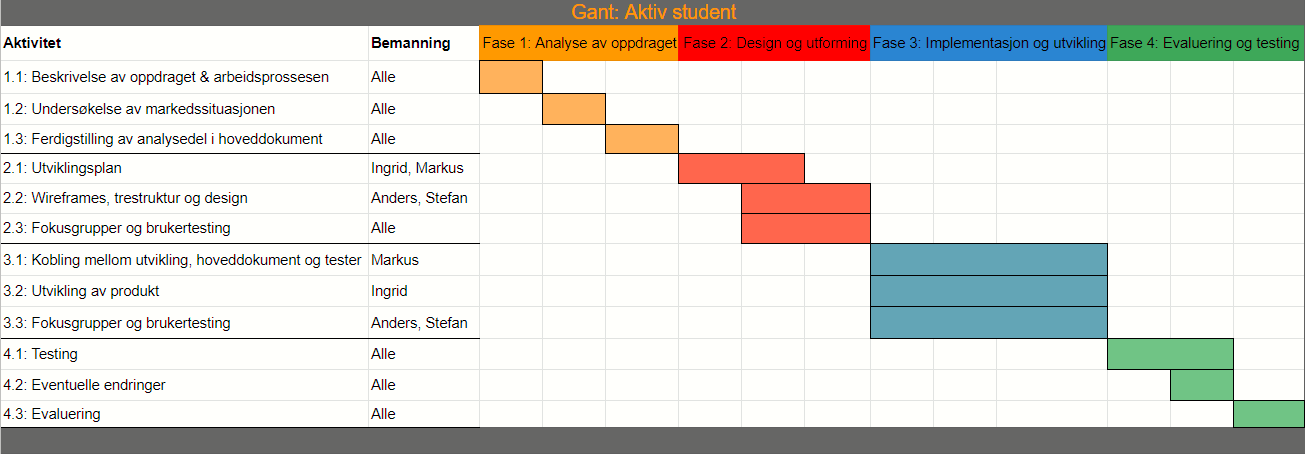
\includegraphics[width=\textwidth]{Illustrasjoner/Gantt.png}
\caption{Gantt-diagram som beskriver oppgaver som skal gjøres og bemanning på de forskjellige delene av prosjektet}
\label{fig:Gantt}
\end{figure}

Gantt diagrammet i figur~\ref{fig:Gantt} er laget for å illustrere de forskjellige hoved-arbeidsoppgavene som må gjennomføres i prosjektet. Diagrammet beskriver punktvis de forskjellige oppgavene som er forklart i hver sin fase av hoveddokumentet og hvilke gruppemedlemmer som har hatt hovedansvar for disse. Gantt-diagrammets formål er å illustrere arbeidsfordeling og skape en bedre oversikt i prosjektet.   

\begin{figure}[H]
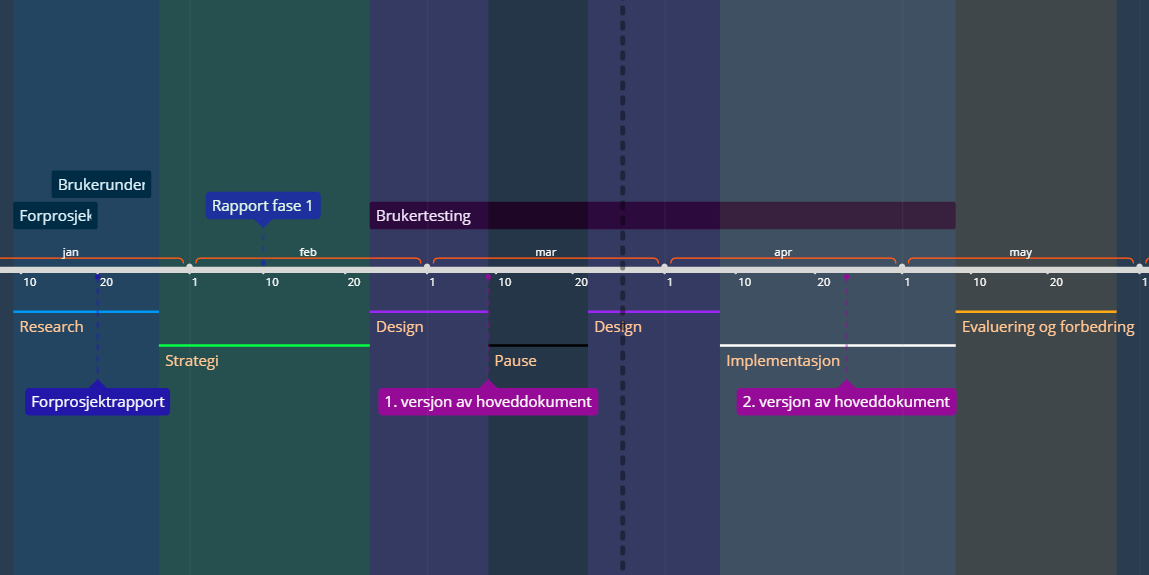
\includegraphics[width=\textwidth]{Illustrasjoner/tidslinje-revidert-igjen.png}
\caption{Tidslinje over prosjektarbeidet}
\label{fig:tidslinje}
\end{figure}

Tidslinjen i figur~\ref{fig:tidslinje} illustrerer de forskjellige fasene i prosjektet og når prosjektgruppen tenker å gjennomføre disse. Tidslinjen er utformet av gruppen i et nett-verktøy som heter TimeGraphics.\footnote{https://time.graphics/line/342770} Her vises det at de fem fasene i Informasjonsarkitektur: research, strategi, design, implementasjon og evaluering \& forbedring, er brukt som grunnlag for strukturering av prosjektarbeidet. Viktige frister i løpet av prosjektet er også lagt inn i tidslinjen.

% skrive om hva som ble gjort under hver fase %

\section*{Samarbeid}

Hvordan fungerte gruppearbeidet?

Hvordan fungerte samarbeidet med oppdragsgiver og veileder?
    
Hva synes du om resultatene, nådde dere målene dere satte dere?

Kunne noe vært gjort bedre/anderledes? 

\section*{Konklusjon}

Her skal du oppsummere i noen få setninger hvordan du vurderer prosjektet som helhet fra et overordnet perspektiv.

\end{document}
